\documentclass[14pt]{extbook}
\usepackage{multicol, enumerate, enumitem, hyperref, color, soul, setspace, parskip, fancyhdr} %General Packages
\usepackage{amssymb, amsthm, amsmath, latexsym, units, mathtools} %Math Packages
\everymath{\displaystyle} %All math in Display Style
% Packages with additional options
\usepackage[headsep=0.5cm,headheight=12pt, left=1 in,right= 1 in,top= 1 in,bottom= 1 in]{geometry}
\usepackage[usenames,dvipsnames]{xcolor}
\usepackage{dashrule}  % Package to use the command below to create lines between items
\newcommand{\litem}[1]{\item#1\hspace*{-1cm}\rule{\textwidth}{0.4pt}}
\pagestyle{fancy}
\lhead{Progress Quiz 3}
\chead{}
\rhead{Version C}
\lfoot{3012-8528}
\cfoot{}
\rfoot{Summer C 2021}
\begin{document}

\begin{enumerate}
\litem{
Describe the end behavior of the polynomial below.\[ f(x) = 7(x + 5)^{4}(x - 5)^{7}(x - 9)^{3}(x + 9)^{3} \]\begin{enumerate}[label=\Alph*.]
\begin{multicols}{2}\item 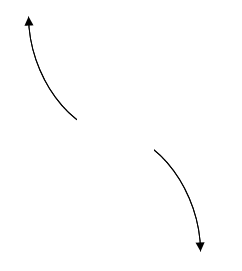
\includegraphics[width = 0.3\textwidth]{../Figures/polyEndBehaviorCopyAC.png}\item 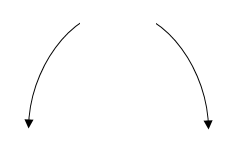
\includegraphics[width = 0.3\textwidth]{../Figures/polyEndBehaviorCopyBC.png}\item 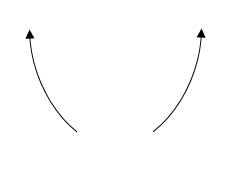
\includegraphics[width = 0.3\textwidth]{../Figures/polyEndBehaviorCopyCC.png}\item 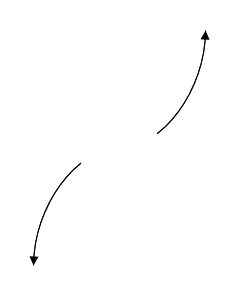
\includegraphics[width = 0.3\textwidth]{../Figures/polyEndBehaviorCopyDC.png}\end{multicols}\item None of the above.
\end{enumerate} }
\litem{
Describe the zero behavior of the zero $x = -5$ of the polynomial below.\[ f(x) = 3(x - 3)^{9}(x + 3)^{7}(x + 5)^{4}(x - 5)^{3} \]\begin{enumerate}[label=\Alph*.]
\begin{multicols}{2}\item 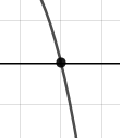
\includegraphics[width = 0.3\textwidth]{../Figures/polyZeroBehaviorAC.png}\item 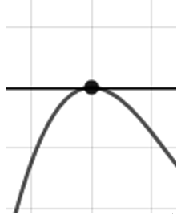
\includegraphics[width = 0.3\textwidth]{../Figures/polyZeroBehaviorBC.png}\item 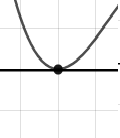
\includegraphics[width = 0.3\textwidth]{../Figures/polyZeroBehaviorCC.png}\item 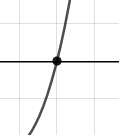
\includegraphics[width = 0.3\textwidth]{../Figures/polyZeroBehaviorDC.png}\end{multicols}\item None of the above.
\end{enumerate} }
\litem{
Which of the following equations \textit{could} be of the graph presented below?
\begin{center}
    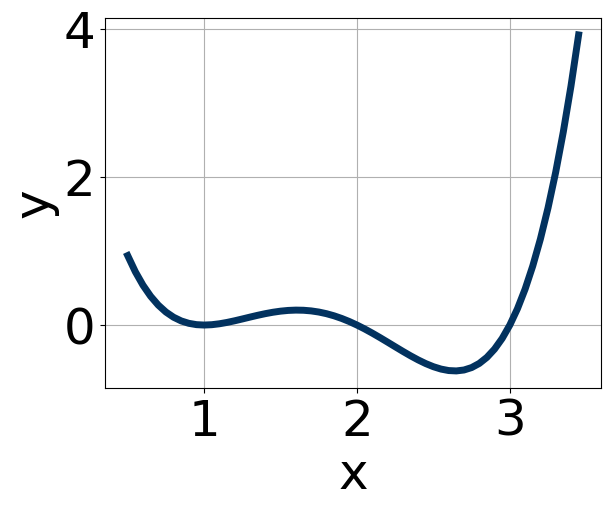
\includegraphics[width=0.5\textwidth]{../Figures/polyGraphToFunctionC.png}
\end{center}
\begin{enumerate}[label=\Alph*.]
\item \( 9(x - 1)^{10} (x - 2)^{8} (x - 3)^{5} \)
\item \( 19(x - 1)^{7} (x - 2)^{10} (x - 3)^{5} \)
\item \( -11(x - 1)^{4} (x - 2)^{11} (x - 3)^{4} \)
\item \( 7(x - 1)^{6} (x - 2)^{11} (x - 3)^{7} \)
\item \( -6(x - 1)^{10} (x - 2)^{11} (x - 3)^{5} \)

\end{enumerate} }
\litem{
Construct the lowest-degree polynomial given the zeros below. Then, choose the intervals that contain the coefficients of the polynomial in the form $x^3+bx^2+cx+d$.\[ 5 + 2 i \text{ and } 4 \]\begin{enumerate}[label=\Alph*.]
\item \( b \in [13, 15], c \in [64, 73], \text{ and } d \in [114, 122] \)
\item \( b \in [-4, 5], c \in [-19, -7], \text{ and } d \in [17, 23] \)
\item \( b \in [-4, 5], c \in [-8, -3], \text{ and } d \in [8, 14] \)
\item \( b \in [-16, -13], c \in [64, 73], \text{ and } d \in [-125, -112] \)
\item \( \text{None of the above.} \)

\end{enumerate} }
\litem{
Which of the following equations \textit{could} be of the graph presented below?
\begin{center}
    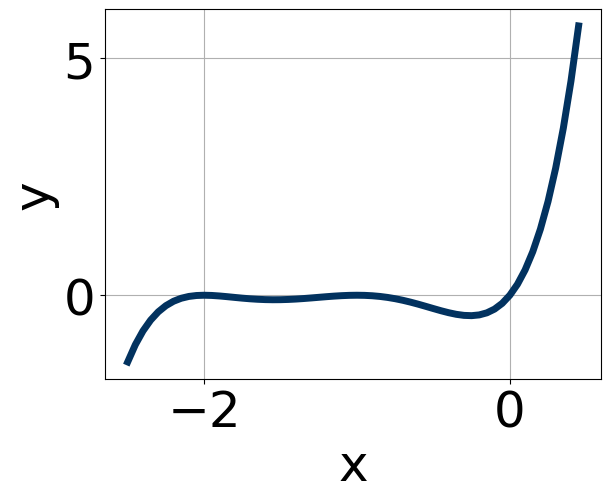
\includegraphics[width=0.5\textwidth]{../Figures/polyGraphToFunctionCopyC.png}
\end{center}
\begin{enumerate}[label=\Alph*.]
\item \( 19x^{5} (x + 1)^{6} (x + 2)^{7} \)
\item \( -14x^{7} (x + 1)^{10} (x + 2)^{4} \)
\item \( 14x^{6} (x + 1)^{10} (x + 2)^{9} \)
\item \( -11x^{4} (x + 1)^{10} (x + 2)^{4} \)
\item \( 2x^{9} (x + 1)^{8} (x + 2)^{10} \)

\end{enumerate} }
\litem{
Describe the end behavior of the polynomial below.\[ f(x) = -4(x - 4)^{3}(x + 4)^{6}(x + 8)^{5}(x - 8)^{5} \]\begin{enumerate}[label=\Alph*.]
\begin{multicols}{2}\item 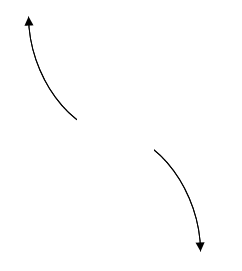
\includegraphics[width = 0.3\textwidth]{../Figures/polyEndBehaviorAC.png}\item 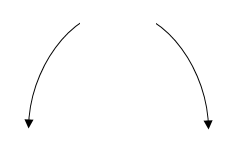
\includegraphics[width = 0.3\textwidth]{../Figures/polyEndBehaviorBC.png}\item 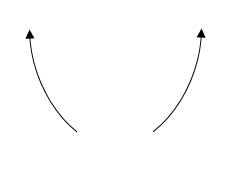
\includegraphics[width = 0.3\textwidth]{../Figures/polyEndBehaviorCC.png}\item 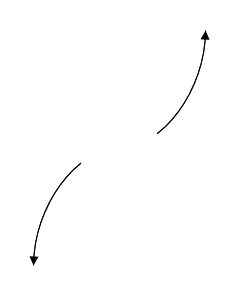
\includegraphics[width = 0.3\textwidth]{../Figures/polyEndBehaviorDC.png}\end{multicols}\item None of the above.
\end{enumerate} }
\litem{
Describe the zero behavior of the zero $x = 9$ of the polynomial below.\[ f(x) = -7(x - 9)^{4}(x + 9)^{7}(x + 2)^{6}(x - 2)^{7} \]\begin{enumerate}[label=\Alph*.]
\begin{multicols}{2}\item 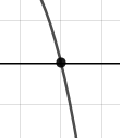
\includegraphics[width = 0.3\textwidth]{../Figures/polyZeroBehaviorCopyAC.png}\item 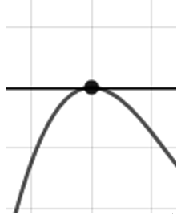
\includegraphics[width = 0.3\textwidth]{../Figures/polyZeroBehaviorCopyBC.png}\item 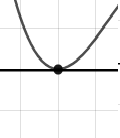
\includegraphics[width = 0.3\textwidth]{../Figures/polyZeroBehaviorCopyCC.png}\item 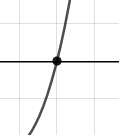
\includegraphics[width = 0.3\textwidth]{../Figures/polyZeroBehaviorCopyDC.png}\end{multicols}\item None of the above.
\end{enumerate} }
\litem{
Construct the lowest-degree polynomial given the zeros below. Then, choose the intervals that contain the coefficients of the polynomial in the form $ax^3+bx^2+cx+d$.\[ \frac{1}{4}, 4, \text{ and } \frac{3}{5} \]\begin{enumerate}[label=\Alph*.]
\item \( a \in [12, 21], b \in [-101, -93], c \in [61, 75], \text{ and } d \in [-15, -8] \)
\item \( a \in [12, 21], b \in [-101, -93], c \in [61, 75], \text{ and } d \in [8, 15] \)
\item \( a \in [12, 21], b \in [-88, -82], c \in [23, 26], \text{ and } d \in [8, 15] \)
\item \( a \in [12, 21], b \in [95, 101], c \in [61, 75], \text{ and } d \in [8, 15] \)
\item \( a \in [12, 21], b \in [69, 77], c \in [-36, -28], \text{ and } d \in [-15, -8] \)

\end{enumerate} }
\litem{
Construct the lowest-degree polynomial given the zeros below. Then, choose the intervals that contain the coefficients of the polynomial in the form $x^3+bx^2+cx+d$.\[ -3 + 2 i \text{ and } 1 \]\begin{enumerate}[label=\Alph*.]
\item \( b \in [-8, -3], c \in [7, 8], \text{ and } d \in [11, 14] \)
\item \( b \in [2, 8], c \in [7, 8], \text{ and } d \in [-16, -8] \)
\item \( b \in [1, 2], c \in [0, 4], \text{ and } d \in [-5, -2] \)
\item \( b \in [1, 2], c \in [-7, 1], \text{ and } d \in [0, 5] \)
\item \( \text{None of the above.} \)

\end{enumerate} }
\litem{
Construct the lowest-degree polynomial given the zeros below. Then, choose the intervals that contain the coefficients of the polynomial in the form $ax^3+bx^2+cx+d$.\[ 4, \frac{-3}{5}, \text{ and } \frac{3}{4} \]\begin{enumerate}[label=\Alph*.]
\item \( a \in [19, 26], b \in [81, 88], c \in [3, 6], \text{ and } d \in [-37, -33] \)
\item \( a \in [19, 26], b \in [76, 78], c \in [-22, -18], \text{ and } d \in [-37, -33] \)
\item \( a \in [19, 26], b \in [-85, -80], c \in [3, 6], \text{ and } d \in [29, 39] \)
\item \( a \in [19, 26], b \in [46, 63], c \in [-101, -94], \text{ and } d \in [29, 39] \)
\item \( a \in [19, 26], b \in [-85, -80], c \in [3, 6], \text{ and } d \in [-37, -33] \)

\end{enumerate} }
\end{enumerate}

\end{document}